\documentclass[12pt,a4wide]{report}

\usepackage{amsthm,amssymb,mathrsfs,setspace,pstricks,amsmath,tikz}%amsmath,%pstcol latexsym,footmisc

\usepackage{play}
\usepackage{epsfig}
%\usepackage[grey,times]{quotchap}
\usepackage[nottoc]{tocbibind}
\renewcommand{\chaptermark}[1]{\markboth{#1}{}}
\renewcommand{\sectionmark}[1]{\markright{\thesection\ #1}}
%

\input xy
%\xyoption{all}


\theoremstyle{plain}
\newtheorem{thm}{Theorem}[section]
\newtheorem{lem}[thm]{Lemma}
\newtheorem{cor}[thm]{Corollary}
\newtheorem{prop}[thm]{Proposition}

\theoremstyle{definition}
\newtheorem{dfn}[thm]{Definition}
\newtheorem{example}[thm]{Example}
\newtheorem{notation}[thm]{Notation}

\theoremstyle{remark}
\newtheorem{remark}[thm]{Remark}
\newtheorem{res}[thm]{Result}
\renewcommand{\baselinestretch}{1.3}




\begin{document}

%\pagenumbering{arabic} \setcounter{page}{1}

% --------------- Title page -----------------------

\begin{titlepage}
\enlargethispage{2cm}

\begin{center}

\vspace*{-1cm}

\textbf{\Large EIGENVALUES OF MATRICES WITH TREE GRAPHS}\\[10pt]

\vspace*{2cm}

A Project Report Submitted \\
for the Course \\[1cm]

{\bf\Large\ MA699 Project}\\[.1in]

\vspace*{1cm}

{\large \emph{by}}\\[.5in]
{\large\bf {Himanshu Prajapati}}\\[5pt]
{\large (Roll No. 222123026)}\\[.55in]

\vfill

\includegraphics[height=3cm]{iitg_logo.eps}

\vspace*{0.5cm}

{\em\large to the}\\[10pt]
{\bf\large DEPARTMENT OF MATHEMATICS} \\[5pt]
{\bf\large \mbox{INDIAN INSTITUTE OF TECHNOLOGY GUWAHATI}}\\[5pt]
{\bf\large GUWAHATI - 781039, INDIA}\\[10pt]
{\it\large April 2024}
\end{center}

\end{titlepage}

\clearpage

% --------------- Certificate page -----------------------
\pagenumbering{roman} \setcounter{page}{2}
\begin{center}
{\Large{\bf{CERTIFICATE}}}
\end{center}
%\thispagestyle{empty}


\noindent
This is to certify that the work contained in this report
entitled {\textbf{``Eigenvalues of Matrices with Tree Graphs"}} submitted by \textbf{Himanshu Prajapati} (\textbf{Roll No: 222123026}) to Department of Mathematics, Indian Institute of Technology
Guwahati towards the requirement of the course \textbf{MA699 Project}
has been carried out by him under my
supervision.

\vspace{4cm}

\noindent Guwahati - 781 039 \hfill (Dr. Sriparna Bandopadhyay)

\noindent April  2024 \hfill Project Supervisor

\clearpage

% --------------- Abstract page -----------------------
\begin{center}
{\Large{\bf{ABSTRACT}}}
\end{center}


The main aim of the project is to study signed digraph and undirected graph of a real square matrix forms a tree or forest structure, we have developed a series of finite, computable methods that provide detailed insights into the sizes and the repeated occurrences of the eigenvalues of the matrix. By using these methods on system designs that are represented as signed directed graphs, we can effectively ensure that these systems are controllable within the framework of linear dynamics.

\clearpage



\tableofcontents
\clearpage
%\listoffigures
%\listoftables
\chapter*{\centerline{List of notations}}
\addcontentsline{toc}{chapter}{List of notations}
\begin{tabular}{ll}
$\mathbb{R}$ & The set of all real numbers\\
%$\CC$ & the set of all complex numbers\\
$\mathbb{R}^n$ & the n-dimensional real Euclidean space\\

$SD(A)$ & Signed digraph associated with matrix $A$\\
$Q(A)$ & The set comprising all matrices having the identical sign pattern as matrix $A$\\
$G(A)$ & Undirected graph associated with matrix $A$\\
$det(A)$ & The determinant of the matrix $A$

\end{tabular}

\pagebreak
\listoffigures  % This command generates the list of figures





\pagenumbering{arabic}
\setcounter{page}{1}

% =========== Main chapters starts here. Type in separate files and include the filename here. ==
% ============================

\input chapter1.tex

\input chapter2.tex

\chapter{Strictly Sinusoidal Trajectories}
\section{Strictly Sinusoidal Trajectories}
\begin{dfn}
	   	A strictly sinusoidal trajectory for the equation  $\dot{x}(t)=\tilde{A}x$ which satisfies $\ddot{x}_i = -x_i$ and $x_i \neq 0$ for all $i$.
\end{dfn}
\begin{lem}
	Suppose $A$ is irreducible, all 2-cycles in $SD(A)$ are positive, and $SD(A)$ contains no $k$-cycle for $k > 2$. Then there exist $\tilde{A} \in Q(A)$ and sinusoidal $x$ solving $\dot{x} = \tilde{A}x$.
\end{lem}

\begin{proof}
	 When all 2-cycles in $SD(A)$ are positive, it implies that for every pair of nodes $i$ and $j$ in the signed digraph with $i \neq j$, the product of the corresponding entries $a_{ij}$ and $a_{ji}$ in $A$ is positive, i.e., $\lambda_i a_{ij} = \lambda_j a_{ji}$ for some positive constants $\lambda_i$ and $\lambda_j$.
	
	As a result, the matrix formed by scaling the entries of $A$ by $\lambda_i^{1/2}$ and $\lambda_j^{-1/2}$ is symmetric and the symmetric matrix has only real eigenvalues. Since $A$ is diagonally similar to this symmetric matrix, it also has only real eigenvalues.
	
	Furthermore, because $A$ has only real eigenvalues, it cannot support a sinusoidal trajectory since sinusoidal functions have purely imaginary eigenvalues.
	
	Therefore, under the given conditions on $SD(A)$, the existence of $\tilde{A}$ and a sinusoidal trajectory $x$ satisfying $\dot{x} = \tilde{A}x$ is not possible.
	
\end{proof}

\begin{lem}
	Suppose $A$ is irreducible and $SD(A)$ has no 1-cycle or $k$-cycle, $k > 2$, but at least one negative 2-cycle. Then there exist $\tilde{A} \in Q(A)$ and strictly sinusoidal $x$ solving $\dot{x} = \tilde{A}x$.
\end{lem}

\begin{proof}
	We will prove above lemma in a constructive approach.Therefore, suppose signed digraph $SD(A)$ contains a negative 2-cycle. The question of existence is resolved by showing that it is always possible to attach straight chains to any subsystem with strictly sinusoidal nodes. In fact, only $\pm\sin t$ and $\pm\cos t$ are required as node values and the entries of $\tilde{A}$ are specified and modified as needed. 
	We will illustrate this with an example, attaching a straight chain to a subsystem  with node set $\{2,3,\ldots, p\}$ with strictly sinusoidal node at node 1. Let's say node 1 has the value $\sin t$. The idea is illustrated in Figure 3.1. We tentatively assign node $p$ the value $\cos t$ if $p$ is even, or $\sin t$ if $p$ is odd. Then we'll set $|\tilde{a}_{p,p-1}| = 1$, so that the sign of $\tilde{a}_{p,p-1}$ determines whether node $p-1$ in $\dot{x} = \tilde{A}x$ is $\pm\dot{x_p}$, that is $\pm \sin t$ if $p$ is even, $\pm \cos t$ if $p$ is odd.
	
	
	Consider the equation at row $p-1$. Specifying either $|\tilde{a}_{p-1,p-2}| = |\tilde{a}_{p-1,p-2}| = 1/2$ or $|\tilde{a}_{p-1,p}| = 1$, $|\tilde{a}_{p-1,p-2}| = 2$, as needed according to edge signs, allows us to keep $x_{p-1} = \pm \dot{x_p}$. This procedure extends down to row 1 of $\dot{x} = Ax$. If there's a sign inconsistency at row 1, we start over with the opposite sign for node $p$ to correct it. If node 1 is $\cos t$, we adjust our strategy accordingly, assigning node $p$ the value $\sin t$ for even $p$ or $\cos t$ for odd $p$, and finally, we adjust the magnitudes of $\tilde{a}_{1j}$ as necessary.
\end{proof}

\begin{figure}[h]
	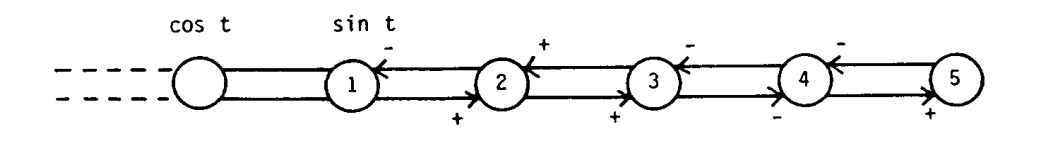
\includegraphics[height=2.0cm]{figure2.png}
	\caption{An illustration of the idea of the proof of Lemma 2. Attachment of a staright chain with node set $\{2,3,4,5\}$ to subsystem at node 1.} 
\end{figure}

\begin{example}
	
%	Consider a example with matrix A of order 5 which satisfying above property of lemma. Now we have to find $\tilde{A} \in Q(A)$ and strictly sinusoidal x satisfyying $\dot{x}=\tilde{A}x$.
%	To find we use above algorithm of proof.  Consider attachment of a straight chain with node set $\{2,3,\ldots, 5\}$ to a subsystem with strictly sinusoidal node values at node 1. Assume node 1 has the value $\sin t$.
%	So,
%	\begin{center}
%		$\tilde{A}=$
%		$\begin{bmatrix}
%			0& a_{12} & 0& 0 &0\\
%			a_{21}& 0& a_{23} & 0& 0\\
%			0 & a_{32}& 0 & a_{34}& 0\\
%			0& 0 & a_{43}& 0 & a_{45}\\
%			0 &0 &0 &a_{54} & 0
%		\end{bmatrix}$
%	\end{center}
%	Now, Solving the system  $\dot{x} = \tilde{A}x$, so
%	\begin{center}
%		$\begin{bmatrix}
%			0& a_{12} & 0& 0 &0\\
%			a_{21}& 0& a_{23} & 0& 0\\
%			0 & a_{32}& 0&  a_{34}& 0\\
%			0& 0 & a_{43}& 0 & a_{45}\\
%			0 &0 &0 &a_{54} & 0
%		\end{bmatrix}$
%	 $\begin{bmatrix}
%	 	x_1 \\
%	 	x_2 \\
%	 	x_3 \\
%	 	x_4 \\
%	 	\sin t \\
%	 \end{bmatrix}$
%	 =
%	 $\begin{bmatrix}
%	 	\dot{x_1} \\
%	 	\dot{x_2}\\
%	 	\dot{x_3}\\
%	 	\dot{x_4}\\
%	 	\cos t \\
%	 \end{bmatrix}$
%	\end{center}
%
%  Equating the row fifth equation we get $a_{54}x_4=\cos t$.By the algorithm of the proof let tentatively set $a_{54}=1$ we get $x_4=\cos t$.
%  
%  Again solving the row 4 equation we get $a_{43}x_3 +a_{45} \sin t= -\sin t$. So,let node value of node 3 is $\sin t$ so choose $a_{43} =-1$ and $a_{45} =-2$ to satisfy equation.
%  
%  Similarly doing for node 3, equating the equation at row 3, we get  $a_{32}x_2 +a_{34} \cos t= -\cos t$. So, let node value of node 2 is $-\cos t$ so choose $a_{32} =1$ and $a_{34} =2$ to satisfy equation.
%  
%  Again solving the row 2 equation we get $a_{21}x_1 +a_{23} \sin t= \sin t$. So,let node value of node 1 is $\sin t$ so choose $a_{21} =1/2$ and $a_{23} =1/2$ to satisfy equation.
%  
%  Lastly solving for row 1 equation, we get $a_{12}(-\cos t) = \cos t$ so choose $a_{12}=-1$ to satisfy row equation. Hence we get,
%  \begin{center}
%  	$\tilde{A}=$
%  	$\begin{bmatrix}
%  		0& -1 & 0& 0 &0\\
%  		1/2& 0& 1/2 & 0& 0\\
%  		0 & 1 & 0& 2 & 0\\
%  		0& 0 & 1& 0 & -2\\
%  		0 &0 &0 &1 & 0
%  	\end{bmatrix}$
%  and $x=$
%   $\begin{bmatrix}
%  	\sin t \\
%  	-\cos t \\
%  	\sin t \\
%  	\cos t \\
%  	\sin t \\
%  \end{bmatrix}$
%  \end{center}
%and satisfying equation;
% \begin{center}
%
%	$\begin{bmatrix}
%		0& -1 & 0& 0 &0\\
%		1/2& 0& 1/2 & 0& 0\\
%		0 & 1 & 0& 2 & 0\\
%		0& 0 & 1& 0 & -2\\
%		0 &0 &0 &1 & 0
%	\end{bmatrix}$
%	$\begin{bmatrix}
%		\sin t \\
%		-\cos t \\
%		\sin t \\
%		\cos t \\
%		\sin t \\
%	\end{bmatrix}$
% =
%$\begin{bmatrix}
%	\cos t \\
%	\sin t\\
%	\cos t\\
%	-\sin t\\
%	\cos t \\
%\end{bmatrix}$
%\end{center}

Consider an example with matrix $A$ of order 5 that satisfies the property of the lemma. Our goal is to find $\tilde{A} \in Q(A)$ and a strictly sinusoidal vector $x$ satisfying $\dot{x}=\tilde{A}x$. To achieve this, we employ the algorithm outlined in the proof.

Let's start by attaching a straight chain with node set $\{2,3,\ldots, 5\}$ to a subsystem with strictly sinusoidal node values at node 1, where node 1 has the value $\sin t$. We represent $\tilde{A}$ as:

\[
\tilde{A} = 
\begin{bmatrix}
	0 & a_{12} & 0 & 0 & 0 \\
	a_{21} & 0 & a_{23} & 0 & 0 \\
	0 & a_{32} & 0 & a_{34} & 0 \\
	0 & 0 & a_{43} & 0 & a_{45} \\
	0 & 0 & 0 & a_{54} & 0
\end{bmatrix}
\]

Solving the system $\dot{x} = \tilde{A}x$, we have:

\[
\begin{bmatrix}
	0 & a_{12} & 0 & 0 & 0 \\
	a_{21} & 0 & a_{23} & 0 & 0 \\
	0 & a_{32} & 0 & a_{34} & 0 \\
	0 & 0 & a_{43} & 0 & a_{45} \\
	0 & 0 & 0 & a_{54} & 0
\end{bmatrix}
\begin{bmatrix}
	x_1 \\
	x_2 \\
	x_3 \\
	x_4 \\
	\sin t
\end{bmatrix}
=
\begin{bmatrix}
	\dot{x_1} \\
	\dot{x_2} \\
	\dot{x_3} \\
	\dot{x_4} \\
	\cos t
\end{bmatrix}
\]

Equating the fifth row equation, we find $a_{54}x_4=\cos t$. Setting $a_{54}=1$, we obtain $x_4=\cos t$. 

Solving the row 4 equation yields $a_{43}x_3 + a_{45} \sin t = -\sin t$. Choosing the node value of node 3 is $\sin t$, we choose $a_{43} = -1$ and $a_{45} = -2$ to satisfy the equation.


Similarly, we solve the row 3 equation by equating it to $a_{32}x_2 +a_{34} \cos t= -\cos t$. Choosing the node value of node 2 to be $-\cos t$, we set $a_{32} = 1$ and $a_{34} = 2$ to satisfy the equation.

Continuing, we solve the row 2 equation by setting it equal to $a_{21}x_1 +a_{23} \sin t= \sin t$. We choose the node value of node 1 as $\sin t$, thus we set $a_{21} = 1/2$ and $a_{23} = 1/2$ to satisfy the equation.

Finally, solving the row 1 equation, we have $a_{12}(-\cos t) = \cos t$. To satisfy this equation, we set $a_{12}=-1$.

 Hence, after completing all the steps, we obtain:
\begin{center}
	$\tilde{A}=
	\begin{bmatrix}
		0 & -1 & 0 & 0 & 0 \\
		1/2 & 0 & 1/2 & 0 & 0 \\
		0 & 1 & 0 & 2 & 0 \\
		0 & 0 & 1 & 0 & -2 \\
		0 & 0 & 0 & 1 & 0
	\end{bmatrix}$
	and $x=
	\begin{bmatrix}
		\sin t \\
		-\cos t \\
		\sin t \\
		\cos t \\
		\sin t
	\end{bmatrix}$
\end{center}

This $\tilde{A}$ and $x$ combination satisfies the equation;
 \begin{center}
		$\begin{bmatrix}
				0& -1 & 0& 0 &0\\
				1/2& 0& 1/2 & 0& 0\\
				0 & 1 & 0& 2 & 0\\
				0& 0 & 1& 0 & -2\\
				0 &0 &0 &1 & 0
			\end{bmatrix}$
		$\begin{bmatrix}
				\sin t \\
				-\cos t \\
				\sin t \\
				\cos t \\
				\sin t \\
			\end{bmatrix}$
	 =
	$\begin{bmatrix}
			\cos t \\
			\sin t\\
			\cos t\\
			-\sin t\\
			\cos t \\
		\end{bmatrix}$
		\end{center}
\end{example}

\begin{thm}
	Suppose $A$ is irreducible and $SD(A)$ has no $k$-cycle, $k > 2$. If there exists a strictly sinusoidal trajectory $x$ solving $\dot{x} = \tilde{A}x$ for some $\tilde{A} \in Q(A)$ then $SD(A)$ has at least one negative 2-cycle and $SD(A)$ is not $\lambda$-consistent.
\end{thm}


\begin{proof}

	Suppose we have a matrix $\tilde{A}$ that belongs to the qualitative class of $A$, denoted as $Q(A)$, along with a strictly sinusoidal trajectory $x$ characterized by certain constants ${\lambda_j}$. Let's assume there exists a 1-cycle at node $i$ within the system. Now, consider the quantity $\Lambda$, defined as $\Lambda = \sum_{i=1}^n \lambda_i x_i^2/2$. for all nodes $i$.
	
	If the signed digraph $SD(A)$ were to be $\lambda$-consistent, then along the trajectory $x$, the derivative of $\Lambda$ would be calculated as $\dot{\Lambda} = \sum_{i=1}^n \lambda_i\tilde{a_{ii}} x_i^2$, which must be greater than zero. However, this contradicts the periodicity property, where $\Lambda(x(t))$ is equal to $\Lambda(x(t+2\pi))$. Lemma 1 concludes that $SD(A)$ must indeed contain a negative 2-cycle.
	
\end{proof}

\begin{cor}
	If $A$ is irreducible and $SD(A)$ has no $k$-cycle, $k > 2$, and exactly one 1-cycle, then no $\tilde{A} \in Q(A)$ admits a strictly sinusoidal trajectory.
\end{cor}

\begin{proof}
	Given these conditions, $SD(A)$ is $\lambda$-consistent, as per Theorem 3.1.5, which effectively rules out the existence of a strictly sinusoidal trajectory.
\end{proof}


\chapter{Constant Trajectories}
\section{Introduction}
In our investigation of solutions to $Ax = 0$, where $x$ is non-zero but some $x_i = 0$, we focus on cases where $n > 2$, excluding the trivial scenario of $n = 1$ where $A$ reduces to the zero matrix. Assuming the irreducibility of $A$ and the absence of cycles longer than 2 in $SD(A)$, if $Ax = 0$ and $x \neq 0$, we can divide the signed digraph $SD(A)$ and the graph $G(A)$ into distinct subgraphs.

To achieve this partitioning, we introduce the concept of a white block, which represents a maximal connected subgraph of nodes in $SD(A)$ corresponding to non-zero components of $x$. Nodes not included in white blocks are labeled as black and form part of black blocks.

This partitioning scheme can be understood through what we term as a "color test".

\section{Constant Trajectories and 0-coloring}
\begin{dfn}
	A constant trajectory $x(t) \in \mathbb{R}^n$ for $\dot{x}_i = \sum_{j=1}^n a_{ij}x_j$ satisfies $\dot{x}_i = 0$ and $x_i \neq 0$ for some $i$.
\end{dfn}
\begin{dfn}
	 A 0-coloring is a scheme for coloring all nodes of $SD(A)$ which has no $k$-cycle, $k > 2$, black or white, so that:
	\begin{enumerate}
		\item no black node is a neighbor of exactly one white node;
		\item each maximal white block as a subgraph is either: a single undistinguished node; or a digraph which has at least two nodes, which has each end node distinguished, and which is not $\lambda$-consistent.
	\end{enumerate}
\end{dfn}

\begin{example}
Consider the matrix 
\begin{center}

$\tilde{A}=
\begin{bmatrix}
	3 & 0 & -3 & 0 & 0 \\
	0 & 1 & -2 & 2 & 0 \\
	-2 & 1 & 2 & 0 & 0 \\
	0 & 3 & 0 & 0 & 0 \\
	0 & 0 & 0 & 0 & 0 \\
\end{bmatrix}$
and let 
$x=
\begin{bmatrix}
	1 \\
	0 \\
	1 \\
	1 \\
	0 \\
\end{bmatrix}$
\end{center}
be a solution corresponding to the equation $Ax=0$. Thus, we color nodes $\{1,3,4\}$ white since the corresponding $x_i$ values for nodes $\{1,3,4\}$ are non-zero. Conversely, nodes $\{2,5\}$ are colored black, indicating that the corresponding $x_i$ values for these nodes are zero. Additionally, this coloring satisfies the criteria of 0-coloring, as node 2 is a neighbor of two white nodes, i.e., nodes 3 and 4.
\begin{center}
	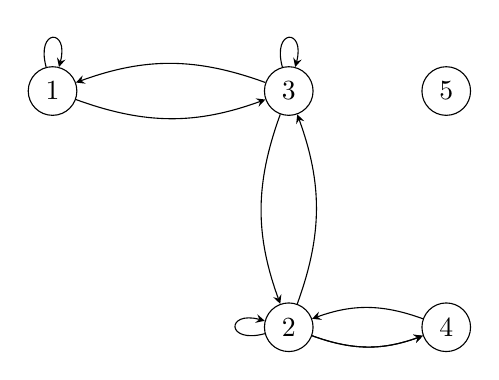
\begin{tikzpicture}[>=stealth]
		% Nodes in a circle
		\node[circle, draw] (1) at (0,0) {1};
		\node[circle, draw] (2) at (3,-3) {2};
		\node[circle, draw] (3) at (3,0) {3};
		\node[circle, draw] (4) at (5,-3) {4};
		\node[circle, draw] (5) at (5,0) {5};
		
		% Edges
		\draw[->] (1) to[bend right=20] (3);
		\draw[->] (2) to[bend right=20] (4);
		\draw[->] (1) to[loop above] (1);
		\draw[->] (3) to[loop above] (3);
		\draw[->] (2) to[loop left] (2);
		
		\draw[->] (2) to[bend right=20] (3);
		\draw[->] (3) to[bend right=20] (2);
		
		\draw[->] (3) to[bend right=20] (1);
		\draw[->] (2) to[bend right=20] (4);
		
		\draw[->] (4) to[bend right=20] (2);
		
	\end{tikzpicture}
\end{center}

\end{example}
\begin{thm}
	Suppose $A$ is an irreducible matrix of order $\geq 2$ and $SD(A)$ contains no $k$-cycle, $k > 2$. Then there exists $\tilde{A} \in Q(A)$ and a vector $x \neq 0$ satisfying $\tilde{A}x = 0$ if and only if $SD(A)$ admits a 0-coloring with at least one white node.
\end{thm}

\begin{proof}
	 First, we are going to prove in a forward direction i.e, $SD(A)$ admits a 0-coloring with at least one white node.
	 Suppose, $n \geq 2$, and we have a non-zero solution $x$ to the equation $Ax = 0$, with the constraint $x \neq 0$. We proceed by coloring all nodes corresponding to non-zero entries in $x$ as white, while the remaining nodes are colored black.
	
   	When all $x_i \neq 0$, Theorem 1 implies condition (ii) is satisfied, as all nodes are white. However, in case where both black and white nodes exist, we need to ensure condition (i) holds true. This condition becomes evident when we examine the equation corresponding to the $j$th row in $Ax = 0$ for some $x_j = 0$. we see condition (i) must be fulfilled.
	
	Each white block represents a subsystem of equations $\bar{A}\bar{x}=0$ within $Ax = 0$, adhering to the conditions outlined in Theorem 1. Consequently, every white block must fulfill condition (ii) to maintain consistency with the theorem's requirements.
	
	Now, let's consider the \textbf{converse} scenario: assume $SD(A)$ admits a 0-coloring with at least one white node. Here's how we construct a non-zero vector $x$ that satisfies $\tilde{A}x = 0$.
	
	We begin by examining the subsystem of equations $\tilde{A}x = 0$ associated with a white block. According to Theorem 1, such a subsystem has a solution where each component is non-zero. We define the components of the complete vector $x$ accordingly.
	
	Suppose node $j$ is black and connected to a node within this white block. By condition (i), node $j$ must be linked to other white nodes $k_1, k_2, \ldots, k_q$, where $q \geq 1$. We assign arbitrary positive values to $|\tilde{a}_{jk_{i}}|$ and choose non-zero ${x_{k_i}}$ values that satisfy the $j$th row equation in $\tilde{A}x = 0$. Using the idea of Theorem 2.1.2, we extend these $x$-values throughout their respective white blocks. Given that $G(A)$ forms a tree, we can systematically extend these values to all white nodes and black nodes connected to white nodes.
	
	We assign arbitrary magnitudes to all other entries in $\tilde{A}$ corresponding to edges in $SD(A)$ originating from black nodes, while setting the components of $x$ corresponding to black nodes to zero. This process completes the construction of $\tilde{A}$ and $x$ satisfying $\tilde{A}x = 0$ with $x \neq 0$.

\end{proof}
\begin{example}
	Let's consider the scenario where $SD(A)$ allows a 0-coloring with at least one white node. We aim to find a non-zero solution $x$ satisfying $Ax = 0$. We begin by examining the subsystem of equations $Ax = 0$ associated with a white block, comprising nodes $\{1,3\}$, assuming they form the maximal white block. Additionally, nodes 4 and 6 are also white but are undistinguished nodes. According to Theorem 2.1.2, such a subsystem has a non-zero solution for each component. Let nodes $\{2,5\}$ be black, and node 2 is linked to white nodes $\{1,3,4,6\}$.
	
	We construct the matrix $\tilde{A}$ as follows:
	\begin{center}
		$\tilde{A}=$
		$\begin{bmatrix}
			3 & 0 & -3 & 0 & 0 & 0\\
			0 & \tilde{a}_{22} & \tilde{a}_{23} & \tilde{a}_{24} & 0 & \tilde{a}_{26}\\
			-2 & \tilde{a}_{32} & 2 & 0 & 0 & 0\\
			0 & \tilde{a}_{42} & 0 & 0 & 0 & 0\\
			0 & 0 & 0 & 0 & 0 & 0\\
			0 & \tilde{a}_{62} & 0 & 0 & 0 & 0\\
		\end{bmatrix}$
	\end{center}
	And let $x$ be:
	\begin{center}
		$x=$
		$\begin{bmatrix}
			1 \\
			0 \\
			1 \\
			x_4 \\
			0 \\
			x_6
		\end{bmatrix}$
	\end{center}
	
	Node 4 is connected to other white nodes 4 and 6. We choose arbitrary positive values for $|\tilde{a}_{24}|$ and $|\tilde{a}_{24}|$ and determine $x_4$ and $x_6$ so that they satisfy the 2nd row equation in $\tilde{A}x=0$. We assign arbitrary magnitudes to all other entries in $\tilde{A}$ corresponding to edges originating from black nodes, while setting the components of $x$ corresponding to black nodes to zero. This process completes the construction of $\tilde{A}$ and $x$, ensuring $\tilde{A}x = 0$ with $x \not\equiv 0$. Hence, $\tilde{A}$ and $x$ using the algorithm of the proof are given by:
	\begin{center}
		$\tilde{A}=$
		$\begin{bmatrix}
			3 & 0 & -3 & 0 & 0 & 0\\
			0 & 1 & 4 & -2 & 0 & 1\\
			-2 & 1 & 2 & 0 & 0 & 0\\
			0 & 3 & 0 & 0 & 0 & 0\\
			0 & 0 & 0 & 0 & 0 & 0\\
			0 & -1 & 0 & 0 & 0 & 0\\
		\end{bmatrix}$
and
		$x=$
		$\begin{bmatrix}
			1 \\
			0 \\
			1 \\
			1 \\
			0 \\
			-2
		\end{bmatrix}$
	\end{center}
Its associated signed digraph is given by;
\begin{center}
	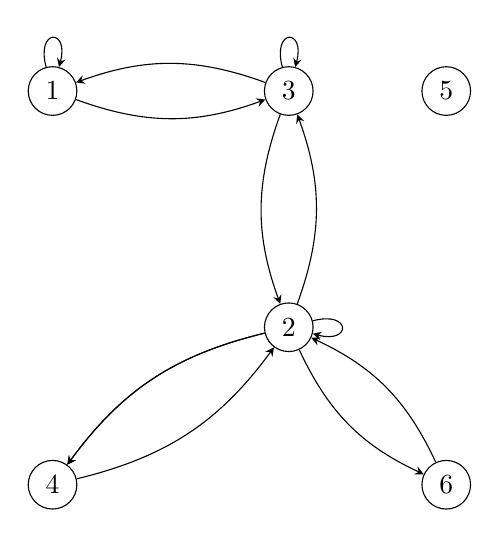
\begin{tikzpicture}[>=stealth]
		% Nodes in a circle
		\node[circle, draw] (1) at (0,0) {1};
		\node[circle, draw] (2) at (3,-3) {2};
		\node[circle, draw] (3) at (3,0) {3};
		\node[circle, draw] (4) at (0,-5) {4};
		\node[circle, draw] (5) at (5,0) {5};
		\node[circle, draw] (6) at (5,-5) {6};
		
		% Edges
		\draw[->] (1) to[bend right=20] (3);
		\draw[->] (2) to[bend right=20] (4);
		\draw[->] (1) to[loop above] (1);
		\draw[->] (3) to[loop above] (3);
		\draw[->] (2) to[loop right] (2);
		
		\draw[->] (2) to[bend right=20] (3);
		\draw[->] (3) to[bend right=20] (2);
		
		\draw[->] (3) to[bend right=20] (1);
		\draw[->] (2) to[bend right=20] (4);
		
		\draw[->] (4) to[bend right=20] (2);
		%\draw[->] (5) to[bend right=20] (4);
		
		\draw[->] (2) to[bend right=20] (6);
		\draw[->] (6) to[bend right=20] (2);
		
	\end{tikzpicture}
\end{center}
\end{example}

\subsection*{Undirected Block graph B(A)}
To explore the presence of multiple eigenvalues in matrix $A$, we introduce the concept of an undirected block graph denoted as $B(A)$. We begin by assuming the existence of a nontrivial 0-coloring scheme for $SD(A)$. In this scheme, we remove from $SD(A)$ all black nodes that are not connected to any white nodes, along with any edges connected to or from these isolated black nodes.

The nodes of $B(A)$ are then composed of the remaining black nodes denoted as ${b_1, b_2, \ldots}$, along with the maximal white blocks denoted as ${w_1, w_2, \ldots}$. An edge ${(b_i, w_j)}$ belongs to $B(A)$ if and only if some node in $b_i$ is connected by a 2-cycle to some node in $w_j$.
Now, we define the concept of branching within $B(A)$. 
\begin{dfn}
	$B(A)$ is branched at a black node if that black node in $B(A)$ is connected to more than two white nodes
\end{dfn} 

\begin{thm}
	Suppose $A$ is irreducible and $SD(A)$ contains no $k$-cycle, $k > 2$. Then 0 is an eigenvalue in at least two Jordan blocks of some $\tilde{A} \in Q(A)$ if and only if $SD(A)$ admits a 0-coloring for which $B(A)$ is branched at a black node.
\end{thm}

\begin{proof}
	Suppose we have a matrix $\tilde{A}$ belonging to the set $Q(A)$, and 0 appears as an eigenvalue in two or more Jordan blocks of $A$. In such a case, there must exist two linearly independent solutions $x$ and $y$ to the equations $\tilde{A}x = \tilde{A}y = 0$.This is because the Jordan Canonical Form (JCF) of a matrix $\tilde{A}$ is a block-diagonal matrix consisting of Jordan blocks, where each Jordan block corresponds to an eigenvalue of $A$. If 0 is an eigenvalue with more than one Jordan block, it implies that there are multiple linearly independent eigenvectors associated with the eigenvalue 0, each corresponding to a different Jordan block.
	 
	We select $x$ in such a way that the number of components with $x_i = 0$ is maximal. If the 0-colorings associated with $x$ and $y$ are identical, then it follows that $x_i = 0$ if and only if $y_i = 0$. By rearranging and renumbering the components, we can arrange for $x_i$ and $y_i$ to be equal and non-zero. Consequently, the 0-coloring associated with $x - y$ would have more zero components than $x$, leading to a contradiction. Therefore, we can assume, without loss of generality, that the 0-coloring associated with $x$ contains the minimal number of white nodes, and that the 0-colorings associated with $x$ and $y$ are distinct.
	
	Consider a scenario where we have a white block in the 0-coloring for vector $x$, denoted as $\bar{x}$, with associated submatrix $\bar{A}$. Let's suppose that this white block is attached at node $i$ to exactly one black node, denoted as node $j$. Such a configuration must always exist. 
	
	Now, let's introduce another vector $y$ with its corresponding 0-coloring. If node $j$ is white in the 0-coloring for $y$, then we can express $\bar{A}\bar{y} + \xi = 0$, where $\xi$ is a vector with only one non-zero entry corresponding to the attachment of node $i$ to the white node $j$. 
	
	Since any vector in the kernel of $\bar{A}$ must be proportional to $\bar{x}$, we can infer that $\bar{y_k} = \alpha \bar{x_k}$ for all nodes in the white block, including node $i$. Upon considering the $i$th row equation, we find $\xi_i = 0$, leading to a contradiction. This contradiction indicates that node $j$ must be black in the 0-coloring for $y$.
	
	By leveraging the tree structure of $G(A)$, this reasoning extends to all nodes that are black in the 0-coloring for $x$ and are attached to white nodes. It demonstrates that no white block of the 0-coloring for $y$ can entirely contain a white block of the 0-coloring for $x$. 
	
	Consequently, if the two colorings differ, it implies that some white block and its adjacent black nodes from the coloring for $x$ lie completely within a black block of the coloring for $y$. 
	
	By coloring a node of $SD(A)$ white if it's white in either the $x$ or the $y$ 0-coloring, and black otherwise, we effectively create a 0-coloring for $SD(A)$. The associated block graph $B(A)$ resulting from this coloring is branched.


	\textbf{For the converse part}, let's consider a 0-coloring for $SD(A)$ exists, and the associated block graph $B(A)$ is branched. Using the reasoning from the first part of Theorem 3, we can construct a vector $y$ and a modified matrix $\tilde{A}$ such that $\tilde{A}y = 0$, ensuring that $y_i \neq 0$ if and only if node $i$ is white in the 0-coloring.
	
	This implies that the components of $y$ corresponding to black nodes are zero, while the edge values from black nodes can take arbitrary values. Within a branched component of $B(A)$, there exists a straight path with white block end nodes. By recoloring all nodes of $SD(A)$ not in this straight path to black, we achieve a distinct 0-coloring.
	
	Using Theorem 4.2.3 once more, we can construct a new vector $x$ (with the same modified matrix $\tilde{A}$) that is not proportional to $y$, but still satisfies $\tilde{A}x = 0$. This process demonstrates how, starting from a branched block graph $B(A)$, we can iteratively generate distinct solutions to the system of equations $\tilde{A}x = 0$ with unique 0-colorings.

\end{proof}

\chapter{Sinusoidal Trajectories}
\begin{dfn}
	A sinusoidal trajectory for our equation satisfies $\ddot{x}_i = -x_i$ and $x_i \not\equiv 0$ ("not the constant function with the value zero") for some $i$.
\end{dfn}
\begin{dfn}
	A Im-coloring is a scheme for coloring all nodes of $SD(A)$ which has no $k$-cycle, $k > 2$, black or white, so that:
	\begin{enumerate}
		\item no black node is a neighbor of exactly one white node;
		\item each maximal white block as a subgraph contains at least one negative $2$-cycle and is not $\lambda$-consistent.
	\end{enumerate}
\end{dfn}
\section{Sinusoidal Trajectories and Im-coloring}
\begin{thm}
		Suppose $A$ is an irreducible matrix of order $> 2$, and $SD(A)$ has no $k$-cycles, $k > 2$. If there exists a sinusoidal trajectory for $\dot{x} = \tilde{A}x$, $x \neq 0$, for some $A \in Q(A)$ then $SD(A)$ admits an Im-coloring with at least one white node.
\end{thm}
\begin{proof}
	If  $\dot{x} = \tilde{A}x$ is a sinusoidal trajectory (x$\equiv$0), color node i white if $x_{i}\equiv0$; otherwise color node i black. Theorem 3.1.5 together with a line of reasoning parallel to that in the first part of the proof of theorem 4.2.3; it becomes evident that such a coloring constitutes a nontrivial Im-coloring. 
\end{proof}
\begin{thm}
	Suppose $A$ is irreducible and $SD(A)$ contains no $k$-cycle, $k > 2$. Then $\iota$ is an eigenvalue in at least two Jordan blocks of some $A \in Q(A)$ if and only if $SD(A)$ admits an Im-coloring for which $B(A)$ is branched at a black node.
\end{thm}
\begin{proof}
	The proof is completely similar to the proof of Theorem 4.2.6(using Theorem 5.1.1)and is omitted.
\end{proof}

%\chapter{Appendix}
\begin{dfn}
	
\end{dfn}


 \nocite{JEFFRIES1988109} \nocite{JEFFRIES19871}

\bibliographystyle{plain}
\bibliography{bib}

\end{document}
